%%% DOCUMENT SETUP %%%
\documentclass[a4]{article}
\usepackage[greek,english]{babel}

%%% LAYOUT %%%
\usepackage{fullpage}
\usepackage[parfill]{parskip}
\usepackage{multicol}
\usepackage{footnote}

%%% GRAPHICS %%%
\usepackage{graphicx}
\usepackage{color}
\usepackage{graphics}
\usepackage{rotating}
\usepackage{subfig}
\usepackage{amsmath}
\usepackage{amssymb}
\usepackage{amscd}
\usepackage{xfrac}
\usepackage{float}
\usepackage{dsfont}

%%% FONT %%%
\usepackage{ifxetex}
\ifxetex
  \usepackage{fontspec}
    \setmainfont{Linux Libertine O}
  \usepackage{xunicode}
  \usepackage{microtype}
\else
  \usepackage[T1]{fontenc}
  \usepackage[latin1]{inputenc}
  \usepackage{times}
  \usepackage{microtype}
\fi

%%% Coding %%%
\usepackage{listings}
\usepackage{pseudocode}

%%% TITLE PAGE %%%
\author{Jeroen Hofman (10194754) \ \ \ \ \ John Tyree (??)  \\[15pt] University of Amsterdam (\textsc{UvA})}

\title{Data Mining Techniques\\
  Assignment 2
		}

\begin{document}
\maketitle
\captionsetup{width=0.8\textwidth}
\lstset{language=Python,breaklines=true,backgroundcolor=\color{white},frame=single}
\thispagestyle{empty}

%%% ABSTRACT %%%
\begin{center}
\begin{abstract}
\end{abstract}
\end{center}

%%% TABLE OF CONTENTS %%%
\newpage
\tableofcontents
\newpage

\section{Task A}
For this task I choose the IJCNN 2011 Social Network Challenge from Kaggle.com running from November 2010 until January 2011. The challenge involved making link predictions on a graph obtained from the popular photo-sharing website Flickr. A large online network was crawled and partitioned to obtain a large training set and a smaller test set which was augmented with a large number of fake edges. The challenge was to predict which of the links was real in the test set and which was not. The algorithm that had to be developed should gave probabilities on the edges in the test set.

The winning group for this challenge was a group by Arvind Narayanan, Elaine Shi and Benjamin Rubenstein. They published a paper about their algorithm, which is quite extensive \cite{Narayanan}. Their algorithm was two-fold and not entirely undisputed; they used their own crawl obtained from the Flickr network to de-anonymize a large part of the edges and then used a variety of algorithms to make predictions on the remaining part of the test set.

The first part of the algorithm is the de-anonymization, which can itself be divided in two steps: seed identification and propagation. The authors had obtained their own graph from Flickr and tried to find correspondences between the graph provided by Kaggle.com (the Kaggle-graph) and their own graph. It turned out that high degree nodes in the graphs have very high correspondence rates and they can be found by techniques like simulated annealing (this is fairly technical and beyond the scope of this assignment). Using these nodes as the seeds it is possible to extent the correspondence between the two graphs by adding a yet unmapped node in one graph and find the most similar node in the other graph. If the nodes are similar enough, they get mapped to each other. This similarity measure is mainly taken from looking at the amount of neighboring nodes in the Kaggle-graph that already correspond with nodes in the Flickr-graph and then looking at nodes in the Flickr-graph which are also connected with these nodes. The details are not trivial since only partial edge information is available. Nevertheless the authors were able to achieve a 64.7\% coverage with just this first step, with an accuracy of 95.2\% (the accuracy is obtained by matching the prediction with the real graph released after the submission deadline).

The second part is the link prediction, in which the key idea is voting. The idea is simple, from the first part they are correspondences of nodes generated, i.e. a node in the Kaggle-graph has a possible correspondence with some nodes in the Flickr-graph. If we look at an edge between two nodes in the Kaggle-graph, there is a number of possible corresponding edges in the Flickr-graph equal to the product of the possible corresponding nodes of both nodes associated with the edge. If none of the edges actually exist in the Flickr-graph, the voting score is zero, if all edges exist, the voting score is 1. On top of this an advanced machine learning algorithm is run with 25 different features, taking into account, node degrees, clustering coefficients, reverse edge searching and more. On top of this a Random Forest classifier was run, which is an advanced and highly efficient algorithm of which further details are described in \cite{randomforest}. The combination of these algorithms gave a very good results, namely an AUC score of 0.981 (with 1 being the maximum).

The main difference of this complicated algorithm compared with other contestants was the large mix of different types of algorithms where most other teams used only a few methods. The de-anonymization part was also somewhat disputed since it was not clear from the original problem description if you were allowed to use de-anonymization, however the jury still approved this approach because of its novelty. The authors goal was also to show that given any anonymous set of partial data, knowing the source is enough to identify large parts of the data.

\section{Task B}
In this task we look briefly at two types of error measures; the mean-squared-error (MSE) and the mean-absolute error (MAE). Let us first clarify something rather confusing, both errors can be defined point-wise, i.e. given predictive value $x_i$ and corresponding real value $y_i$, $1 < i < N$, the errors are defined as:

\begin{align*}
  &\text{MSE} = \frac{1}{N} \sum^N_{i=1} (x_i - y_i)^2 \; \text{and} \\
  &\text{MAE} = \frac{1}{N} \sum^N_{i=1} |x_i - y_i|
\end{align*}

However, we can also regard each $x_i$ as being a sample from some distribution, in which case there is a characteristic $y$ of the distribution for which the error is defined as:

\begin{align*}
  &\text{MSE} = \frac{1}{N} \sum^N_{i=1} (x_i - y)^2 \; \text{and} \\
  &\text{MAE} = \frac{1}{N} \sum^N_{i=1} |x_i - y|
\end{align*}

In this last case it is straightforward to find $y$ such that MSE and MAE are minimized. We do this by taking the derivative of MSE/MAE with respect to $y$ and setting it equal to zero, giving the following equations:

\begin{align*}
  &\frac{-2(x_1 - y) + ... + -2(x_n - y)}{n} = \frac{2ny - 2(x_1 + ... + x_n)}{n} = 0 \; \text{(MSE)} \\
  &\frac{\frac{-2(x_1 - y)}{2|x_1 - y|} + ... + \frac{-2(x_n - y)}{2|x_n - y|}}{n} = 0 \; \text{(MAE)}
\end{align*}

In the first case $y = \frac{x_1 + ... + x_n}{n}$ is the solution, for the second case note that $\frac{(x_i - y)}{|x_i - y|}$ is either plus or minus one depending on $y$. The only way in which the total sum is zero is when half of the values of $x_i$ is below $y$ and the other half is above. Hence $y$ is the median of $x_1...x_n$. Hence we conclude that we use the MSE if we are interested in the mean and the MAE if we are interested in the median.

In which case are we interested in what quantity? In the case of a skewed distribution the mean is not as much as an accurate predictor as the median, hence the median is preferred. If the distribution is symmetrical the mean and the median coincide or are almost equal, and hence both errors can be used. So in short, if we want to fit our data to a symmetrical distribution we use the MSE as a measure for the error, if the distribution is non-symmetrical we can use the MAE. The examples are abundant, take for instance the average length of a person, this will be normally distributed and hence we want to test our samples against the mean and we can use the MSE as a measure. On the other hand, suppose we measure income, this is a skewed distribution (with outliers to high values) and it is best to use the MAE. This also applies to the point-wise error as defined above, since the data-set can always be transformed such that $y_i = y$ for every $i$. However here it is the spread around the regression line which is either symmetrical or skewed (so allowing for some points to be far from the line). Notice however that the errors are not directly comparable, i.e. a lower MSE than a MAE does not necessarily imply that the spread is more symmetrical.

As a test set we choose a famous data-set in history, namely the iris flower set produced in 1936 by Sir Ronald Fisher \cite{Fischer}. It contains 150 entries with 5 attributes each: the name of the iris flower species, the petal length and width and the sepal length and width. In this small model we investigate whether the sepal length can be predicted given the petal length, width and the sepal width, for a certain species, namely Iris Setosa. We performed both a linear regression as well as a polynomial regression on the data with numerical cross validation. For the linear regression we found the following result:

\begin{equation*}
  \text{sepal length} = 0.660*\text{sepal width} + 0.255*\text{petal length} + 0.135*\text{petal width} + 2.345
\end{equation*}

The latter two parameters are not statistically significant, since their p-values are way too high (0.4 and 0.5). The performance for this relation given above is an RMSE of 0.244 $\pm$ 0.071 and an MAE 0.210 $\pm$ 0.069. Note that the MSE is smaller than the MAE. If we repeat this experiment only taking into account the sepal width, we get:

\begin{equation*}
  \text{sepal length} = 0.691*\text{sepal width}
\end{equation*}

with an RMSE of 0.236 $\pm$ 0.069 and an MAE of 0.199 $\pm$ 0.061, in which case the MSE is smaller than the MAE. As stated before, nothing can be concluded from this, since the error measures are not comparable, they only make more sense in certain distributions of data.

For the polynomial regression we found the following:

\begin{equation*}
  \text{sepal length} = 0.480*\text{sepal width} - 0.034*\text{petal length} - 10.653*\text{petal width}^5 + 3.475
\end{equation*}

with an RSME of 2.006 $\pm$ 2.612 and an MAE of 1.602 $\pm$ 2.066. In this case the MSE is larger than the MAE. The polynomial regression fits much worse than the linear regression. 

\section{Task D}
In this task we investigate the data-set ZAVdataset.csv. The data-set consists of three attributes V, a and z with a total of 5000 entries. If we do an exploratory analysis of the data we see that there is a large amount of clustering. Figure \ref{fig:explore} below shows this clustering for the three possible combinations of parameters. 

\begin{figure}[H]
  \centering
  \subfloat{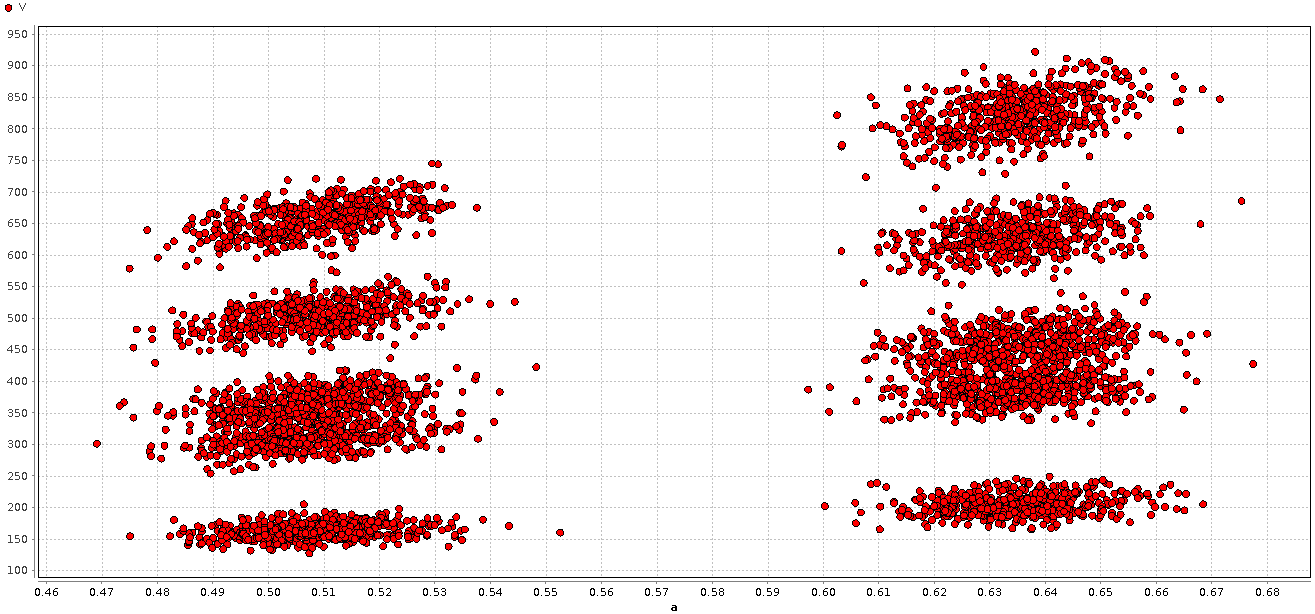
\includegraphics[width=0.6\textwidth]{av.png}}\\
  \subfloat{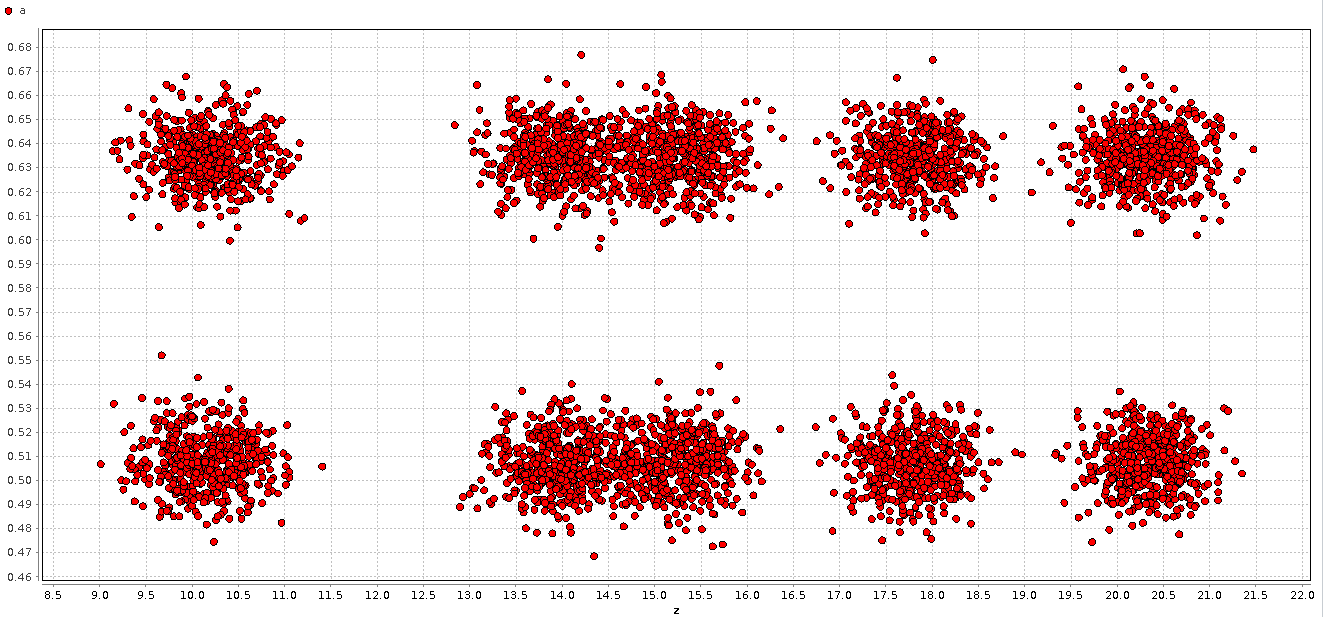
\includegraphics[width=0.6\textwidth]{az.png}}\\  
  \subfloat{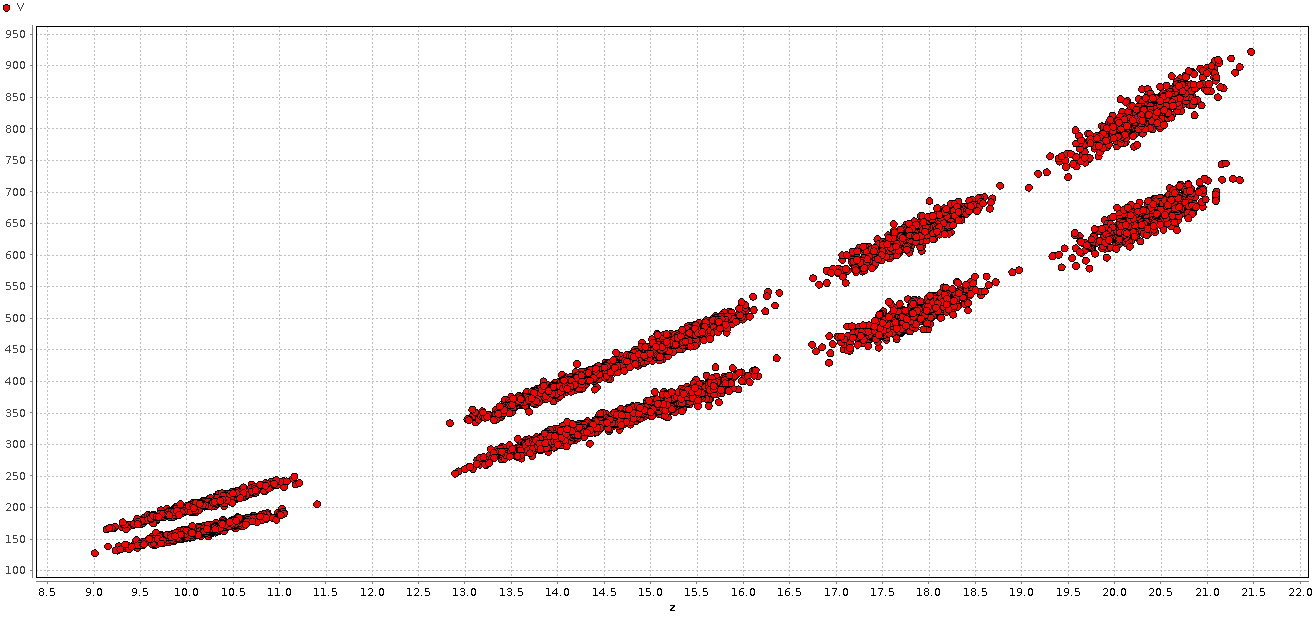
\includegraphics[width=0.6\textwidth]{vz.png}}\\
  \caption{Scatter plots of the data for a against V (top), a against z (middle) and z against V (bottom).}
  \label{fig:explore}
\end{figure}

In order to find the missing attribute names we considered a number of different linear regressions with $V$ as the label. Using the hint from the lecture we also performed linear regression with attributes which are a combination of attributes. We used only the data from the lower 'band' in the bottom plot of figure \ref{fig:explore}. After trying several combinations we found the following linear regression which fits very well:

\begin{equation*}
  V = -0.001z - 0.0001a - 3.142z^2a + 0.007
\end{equation*}

The p-values of all terms except the $z^2a$ term are higher than 0.1 and hence are not statistically significant, hence we can conclude that:

\begin{equation*}
  V = 3.14z^2a
\end{equation*}

is a suitable linear regression. Indeed, this also shows graphically, as figure \ref{fig:pizza} shows below. Note that both solid lines are the same fit but with different intercept term.

\begin{figure}[H]
  \centering
  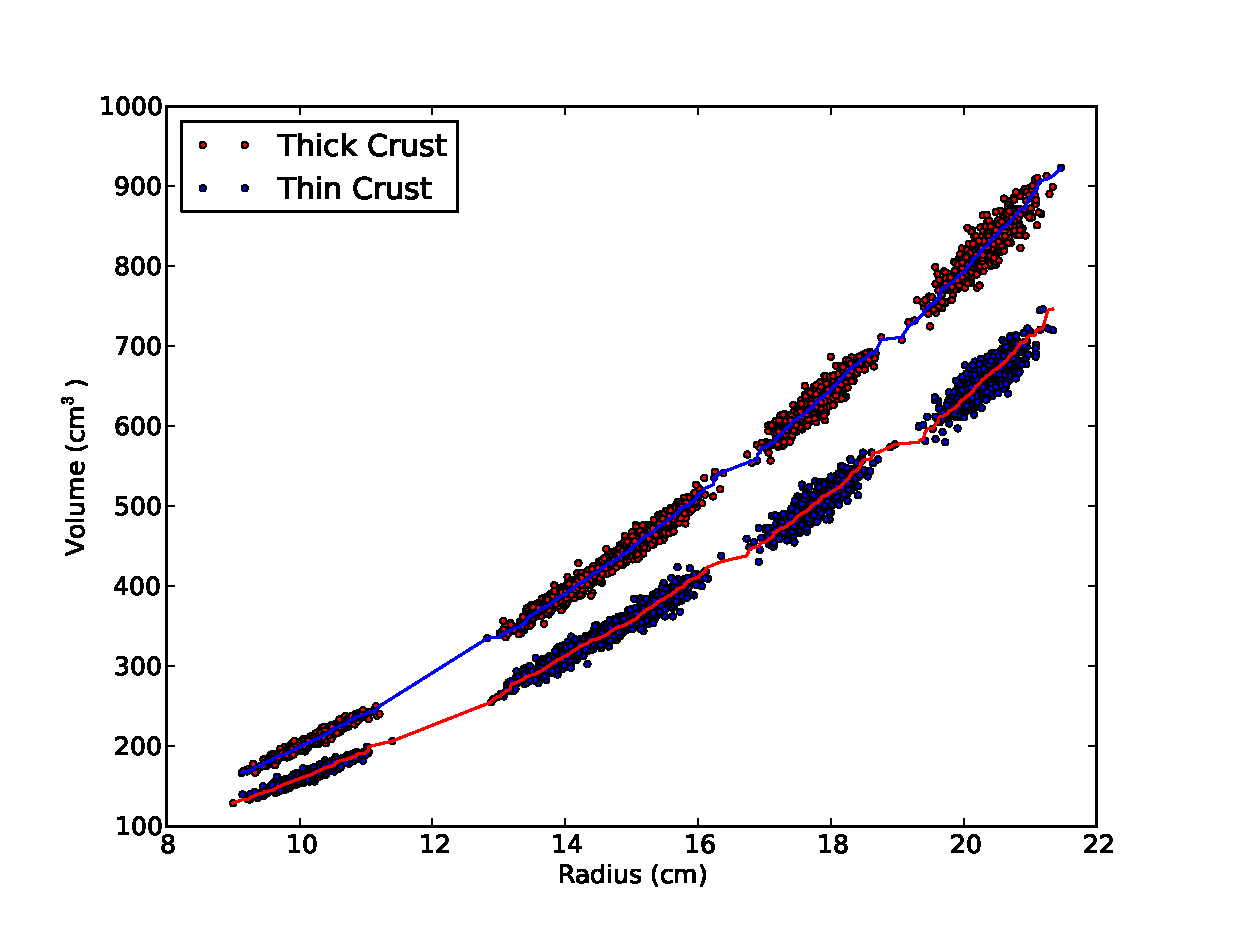
\includegraphics[width=0.7\textwidth]{pizza.eps}
  \caption{The volume of a pizza as a function of its radius, for two different types of crust thickness. The solid line is the fit obtained from the linear regression.}
  \label{fig:pizza}
\end{figure}

From the equation above we can obtain the attribute names, since a formula of the form $\pi r^2h$ gives the volume of a cylinder with radius $r$ and height $h$, so the equation describes the volume of a cylinder, given its radius and height. If we write out the name of the formula in letters we get Pi-z-z-a, which gives the second hint needed to complete the puzzle. Hence the equation above gives the volume of a pizza, given the radius of the pizza $z$ and the crust thickness $h$. 

Returning to the clustering, we can use some simple clustering algorithms to make the clusters more visible. **FIGURE** We see two distinct clusters with respect to the variable $a$, the thickness of the crust. This corresponds to two different types of crust thickness; the Italian crust (thin) and the American crust (thick). Furthermore we see 5 clusters in the $z$ direction, this corresponds with 5 different sizes of the pizza, namely roughly 10, 14, 15.2, 17.7 and 20.5 cm. Converting this to diameter and then to inches this corresponds to roughly 8, 11, 12, 14 and 16 inch, which are the standard sizes for pizzas in large American pizza chains like Dominos or Pizza Hut.

%%% BIBLIOGRAPHY %%%
\begin{thebibliography}{7}
\bibitem{Fischer}
  http://archive.ics.uci.edu/ml/datasets/Iris
\bibitem{Narayanan}
  Narayanan, A., Shi, E. \& Rubinstein, B.I.P. \emph{Link Prediction by De-anonymization: How We Won the Kaggle Social Network Challenge}. Distribution abs/1102.4, 11 (2011).
\bibitem{randomforest}
  Breiman, L., \emph{Random Forests}, Machine Learning 45 (1) (2001).
\end{thebibliography}

\end{document}

%%% Format for lstlisting %%%
%\lstinputlisting{filename.java}
%\begin{lstlisting}
%\end{lstlisting}

%%% Format for multicolumn in table %%%
%\multicolumn{size}{orientation}{}